\documentclass{article}
\usepackage{amsmath}
\usepackage{amsfonts}
\usepackage{graphicx}
\providecommand{\mydet}[1]{\ensuremath{\begin{vmatrix}#1 \end{vmatrix}}}
\providecommand{\myvec}[1]{\ensuremath{\begin{bmatrix}#1 \end{bmatrix}}}
\providecommand{\cbrak}[1]{\ensuremath{\left\{#1\right\}}}
\providecommand{\brak}[1]{\ensuremath{\left(#1\right)}}



\begin{document}

\begin{enumerate}
	\item \textbf{Assertion (A):} Domain of $ y = \cos^{-1}(x) $ is $[-1, 1]$.\\
		\textbf{Reason (R):} The range of the principal value branch of $ y = \cos^{-1}(x) $ is $[0, \pi]$- $\{\frac{\pi}{2}\}$.


\item If $ a = \sin^{-1}\left(\frac{\sqrt{2}}{2}\right) + \cos^{-1}\left(\frac{-1}{2}\right) $ and $ b = \tan^{-1}(\sqrt{3}) + \cot^{-1}\left(\frac{-1}{\sqrt{3}}\right) $, then find the value of $a + b$.


\item Find: $\int \cos^3  x \cdot e^{\log(\sin x)}dx$

\item Find: $\int \frac{1}{5+4x-x^2}dx$	

\item Sand is pouring from a pipe at the rate of $ 15 cm^3/minute$. The falling sand forms a cone on the ground such that the height of the cone is always one- third of the radius of the base. How fast is the height of the sand cone increasing at the instant when the height is $4cm$	 

\item Find the vector equation of the line passing through the point $(2, 3, -5)$ and making equal angles with the co-ordinate axes.

\item Verify whether the function f defined by $f\brak{x} = \begin{cases} x \sin{\left(\frac{1}{x}\right)}, & x \neq 0 \\ 0, & x = 0 \end{cases} $\\
\text{ is continuous at } $x$ = 0 \text{ or not.}


\item Check for differentiability  of the function f defined by $f(x) = |x-5|$, at the point $x = 5$.


\item Find the particular solution of the  differential equation : \\
	$ \frac{dy}{dx} - 2xy = 3x^2e^{x^2} ; y(0)=5 $

\item Solve the following differential equation:\\
	$x^2 dy+y(x+y)dx=0$

\item Find the values of $a$ and $b$ so that the following function is differentiable for all values of $x$  $f\brak{x} = \begin{cases} ax+b, & x>-1 \\ bx^2-3, & x\le -1 \end{cases} $
2
\item Find $ \frac{dy}{dx},$ if $(\cos{x})^y = (\cos{y})^x.$
\item If $\sqrt{1-x^2} + \sqrt{1-y^2} =a(x-y)$, prove that $ \frac{dy}{dx}= \sqrt{\frac{1-y^2}{1-x^2}}.$



\item Evaluate: $\int_{0}^{\pi}\frac{e^{\cos{x}}}{e^{\cos{x}} + e^{-\cos{x}}}dx = 0$

\item Given $\vec{a}=2\hat{i}-\hat{j}+\hat{k}$,$\vec{b}=3\hat{i}-\hat{k}$ and $\vec{a}=2\hat{i}+\hat{j}-2\hat{k}$. Find a vector $\vec{d}$ which is perpendicular to both $\vec{a}$ and $\vec{b}$ and $\vec{c}\cdot\vec{d}=3$ .

\item Bag I contains 3 red and black balls, Bag II contains 5 red and 2 black balls. Two balls are transferred at random from Bag I to Bag II and then a ball is drawn at random from Bag II. Find the probability that the drawn ball is red in colour.


\item Find the co-ordinates of the foot of the perpendicular drawn from the point $(2,3,-8)$ to the line $\frac{4-x}{2} = \frac{y}{6} = \frac{1-z}{3}$.\\
Also, find the perpendicular distance of the given point from the line.

\item Find the shortest distance between the lines $L_{1} \& L_{2}$ given below:\\
	$L_{1}:$ The line passing through $(2,-1,1)$  and parallel to $ \frac{x}{1} = \frac{y}{1}=\frac{z}{3}$\\
		$L_{2}:$  $\vec{r}= \hat{i}+(2\mu + 1)\hat{j}-(\mu + 2)\hat{k}$


\item If $A=\myvec{ 1 & 2 & -3\\2 & 0 & -3\\1 & 2 & 0}$ then find $A^{-1}$ and use it to solve the following system of equations :
	\begin{align*}  x + 2y -3z&= 1\\
		2x-3z & =2\\
                x+ 2y &=3 \end{align*}

\item Find the product of the matrices $\myvec{ 1 & 2 & -3\\2 & 3 & 2\\3 & -3 & 4}$ $\myvec{  -6 & 17 & 13\\14 & 5 & -8\\-15 & 9 & -1}$,then find $AB$ and use it to solve the system of linear equations :
\begin{align*} x - 2y &= 3\\2x - y - z &= 2\\-2y + z &= 3\end{align*}


\item Find the area of the region bounded by the curve $ 4x^2 + y^2 =36$. using integration.


\item Solve the following Linear Programming problem graphically:\\ Maximise $Z=300x + 600y $\\
	Subject to \begin{align*}x + 2y \le 12\\
		2x + y \le 12\\
		x +\frac{5}{4}y \ge 5\\
		x \ge 0 , y \ge 0.\end{align*} 

\item A departmental store sends bills to charge its customers once a month. Past experience shows that 70\% of its customers pay their first month bill in time. The store also found that the customer who pays the bill in time has the probability of 0.8 of paying in time next month and the customer who doesn't pay in time has the probability of 0.4 of paying in time the next month.

Based on the above information, answer the following questions:		
\begin{enumerate}
	\item[(i)] Let $E_{1}$ and $E_{2}$ respectively denote the event of customer paying or not paying the first month bill in time.\\ Find $P(E_{1})$,$P(E_{2})$
	\item[(ii)] Let $A$ denotes the event of customer paying second month's bill in time, then find $P( A|E_{1} ) and P( A |E_{2})$.
	\item[(iii)] Find the probability of customer paying second month's bill in time.
	\item[(iv)] Find the probability of customer paying first month's bill in time if it is found that customer has paid the second month's bill in time.
\end{enumerate}


\item Students of a school are taken to a railway museum to learn about railways heritage and its history\\
	\begin{figure}[h!]
		\centering
		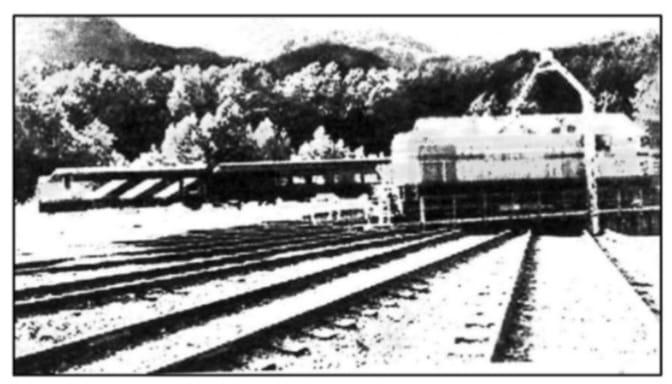
\includegraphics[width=\columnwidth]{images/fig1.jpg}
		\label{fig:image1}
	\end{figure}
	An exhibt in the museum depicted many rail lines on the tack near the railway station. let $L$ be the set of all ral lines on the railwa track and $R$ be the relation on $L$ defined by\\
		$R$={$(l_{1},l_{2}):l_{1} $is parallel to $l_{2}$}\\
	On the basis of the above information, answer the following questions:
\begin{enumerate}
\item Find whether the relation $R$ is symmetric or not.

\item Find whether the relation $R$ is transitive or not.

\item If one of the rail lines on the railway track is represented by the equation $y = 3x + 2$ then find the set of rail lines in $R$ related to it.

\end{enumerate}
\item Let $S$ be the relation defined by $S$ = {$( l_{1},l_{2}):l_{1}$ is perpendicular to $l_{2}$} check whether the relation $S$ is symmetric and transitive.

\item A rectangular visiting card is to contain $24 sq.cm.$ of printed matter. The margins at the top and bottom of the card are to be $1 cm$ and the margins on the left and right are to be cm as shown below:

\newpage
\begin{figure}[h!]
\centering
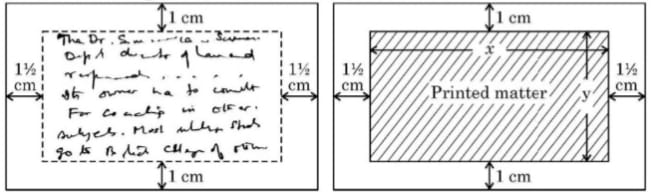
\includegraphics[width=\columnwidth]{images/fig2.jpg}
\label{fig:image2}
\end{figure}

On the basis of the above information, answer the following questions:
\begin{enumerate}
	\item[(i)] Write the expression for the area of the visiting card in terms of $x$.

	\item[(ii)] Obtain the dimensions of the card of minimum area.



\end{enumerate}
\end{enumerate}

\end{document}
